\documentclass[border=10pt]{standalone}
\usepackage{tikz}\usepackage{amsmath}\usetikzlibrary{arrows.meta}
\begin{document}
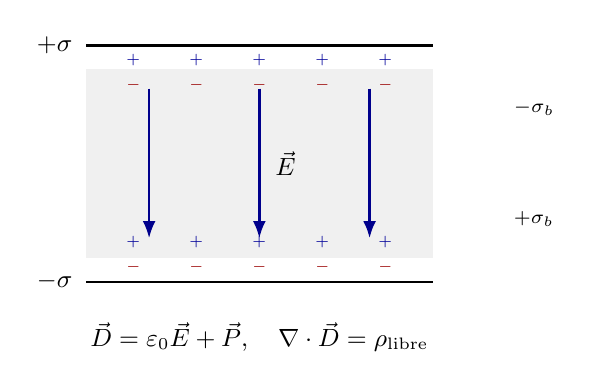
\begin{tikzpicture}[line width=0.9pt,>={Latex[length=2.2mm]}]
  % placas
  \draw[thick] (-2.2,1.5)--(2.2,1.5); \node at (-2.6,1.5){\small$+\sigma$};
  \draw[thick] (-2.2,-1.5)--(2.2,-1.5); \node at (-2.6,-1.5){\small$-\sigma$};
  \foreach \x in {-1.8,-1,-0.2,0.6,1.4} \node[blue!60!black] at (\x+0.2,1.32){\tiny$+$};
  \foreach \x in {-1.8,-1,-0.2,0.6,1.4} \node[red!60!black] at (\x+0.2,-1.32){\tiny$-$};
  % dielectrico
  \fill[black!6] (-2.2,-1.2) rectangle (2.2,1.2);
  % carga ligada
  \foreach \x in {-1.8,-1,-0.2,0.6,1.4} \node[red!60!black] at (\x+0.2,1.0){\tiny$-$};
  \foreach \x in {-1.8,-1,-0.2,0.6,1.4} \node[blue!60!black] at (\x+0.2,-1.0){\tiny$+$};
  \node at (3.1,0.7)[right]{\scriptsize $-\sigma_b$};
  \node at (3.1,-0.7)[right]{\scriptsize $+\sigma_b$};
  % campo
  \foreach \x in {-1.4,0,1.4} \draw[->,blue!55!black,line width=1pt] (\x,0.95)--(\x,-0.95);
  \node at (0,0)[right=2pt]{\small$\vec E$};
  \node at (0,-2.2){\small $\vec D=\varepsilon_0\vec E+\vec P,\quad \nabla\cdot\vec D=\rho_{\text{libre}}$};
\end{tikzpicture}
\end{document}
